\documentclass[border=5pt]{standalone}
\usepackage{tikz}
\usepackage{amsmath}
\usepackage{pgfplots}
\pgfplotsset{compat=1.18}
\begin{document}
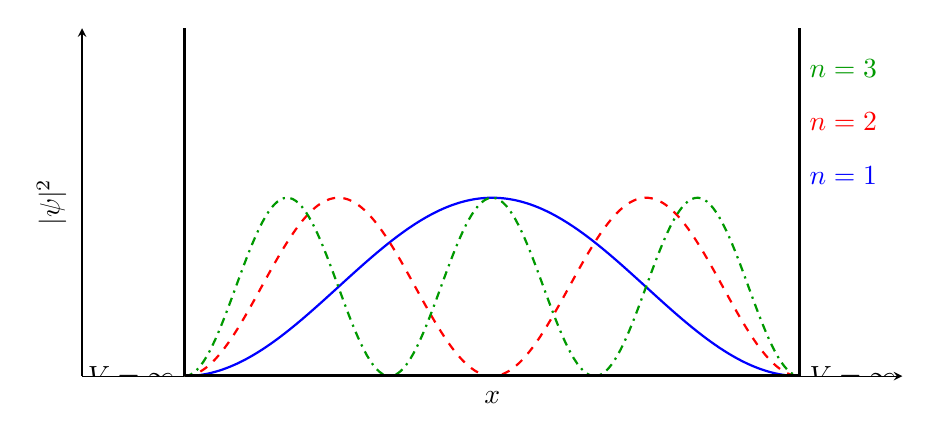
\begin{tikzpicture}
    \begin{axis}[
        width=12cm, height=6cm,
        xlabel={$x$},
        ylabel={$|\psi|^2$},
        xmin=-0.5, xmax=3.5,
        ymin=0, ymax=1.3,
        axis lines=left,
        xtick=\empty,
        ytick=\empty,
        every axis plot/.append style={thick}
    ]
    % n=1
    \addplot[blue,domain=0:3,samples=200] {(2/3)*sin(deg(pi*x/3))^2};
    \node[blue,right] at (axis cs:3,0.75) {$n=1$};
    
    % n=2
    \addplot[red,dashed,domain=0:3,samples=200] {(2/3)*sin(deg(2*pi*x/3))^2};
    \node[red,right] at (axis cs:3,0.95) {$n=2$};
    
    % n=3
    \addplot[green!60!black,dashdotted,domain=0:3,samples=200] {(2/3)*sin(deg(3*pi*x/3))^2};
    \node[green!60!black,right] at (axis cs:3,1.15) {$n=3$};
    
    % 势阱边界
    \draw[very thick] (axis cs:0,0) -- (axis cs:0,1.3);
    \draw[very thick] (axis cs:3,0) -- (axis cs:3,1.3);
    \draw[very thick] (axis cs:0,0) -- (axis cs:3,0);
    
    % 标注
    \node[below] at (axis cs:0,0) {$0$};
    \node[below] at (axis cs:3,0) {$a$};
    \node[left] at (axis cs:0,0) {$V=\infty$};
    \node[right] at (axis cs:3,0) {$V=\infty$};
    \node[below] at (axis cs:1.5,0) {$V=0$};
    \end{axis}
\end{tikzpicture}
\end{document}
